
\documentclass[twocolumn]{article}
\usepackage{cite}
\usepackage{graphicx}
\usepackage{amsmath}
\usepackage{commath}
\usepackage{adjustbox}
%\usepackage[sc]{mathpazo}
\usepackage[margin=0.5in]{geometry}
%\usepackage{multicol}
\usepackage{mathtools}
\usepackage{abstract}
\usepackage[compact]{titlesec}
\DeclareMathOperator{\sech}{sech}
\newcommand{\matr}[1]{\mathbf{#1}}
%\usepackage{placeins}
%\usepackage{textcomp}
\graphicspath{ {H:/} }

\begin{document}

\title {\textbf{Literature Review: Complexity science approach to Atrial Fibrillation}}
\author{Tigany Zarrouk\\ CID: 00823932\\\textbf{Supervisor}: Kim Christensen \\\textbf{Word Count}: 2488.}

\date{}
\maketitle





\begin{abstract}

Modelling Atrial Fibrillation (AF) to ascertain its causes accurately, allowing for effective treatment, has been extensively studied over the past few decades. It is the largest cause of strokes linked with cardiac arrhythmia in aging populations and is due to impaired contractility of the atria in the heart, leading to blood clot formation. Action potential propagation, mediated by ionic species, are seen to be irregular in AF, which causes some atrial myocytes to contract at 300+ times per minute, much faster than healthy hearts which contract at 60-100 times per minute. This beating is regulated by the sinoatrial node which initiates action potentials that propagate through myocytes, causing contractions. Altered refractory period and conduction speed of signals has been seen to promote AF in various models and is caused physically by the fibrosis of cells, reducing the coupling of electrical signals transversally to some myocytes; giving rise to reentry circuits. The most prominent reentry model, the spiral wave model, has been seen to more closely follow clinical and experimental observations than other models of wavefront action. Cellular automata modelling paves the way for large scale simulations of tissue in the heart without the need to solve differential equations, which can be computationally costly. Moore neighbourhoods are seen to be more effective at producing isotropy of spiral waves, reducing flat edges, in rectilinear cellular automata models. Modelling scroll waves, using hybrid cellular automata models, using novel methods to find rotors and replicating the morphology of the heart with its heterogeneities more closely seem to be viable directions for further research. 

\end{abstract}


\section{\textbf{\underline{Introduction}}}

Medical science and the study of disease has been a crucial marker of society's success and development through the ages. Understanding disease gives insights into how to treat and diagnose serious conditions, of which can be fatal. One such condition that has eluded explanation and effective treatment is Atrial Fibrillation (AF), which is the leading cause of Ischaemic stroke in people over 75---seemingly due to incomplete contraction which leads to the formation of blood clots that can travel to the brain \cite{Hart}. It has been known that there are cardiovascular diseases that are predisposed to initiate AF, such as Congestive Heart Failure, Pericarditis and Hypertension through a combination of atrial pressure and dilation, but the precise mechanics are unknown. AF and VF (ventricular fibrillation) are thought to be caused by the breakup of waves of electrical impulses, that induce contraction, into interfering wavelets that produce chaotic behaviour. 

Healthy hearts have a regular, sinus  rhythm which is moderated by the sinoatrial node located in the right atrium of the heart. Fibrillatory activity in the atrium is characterised by a hastened activation of cells: atrial cells activate 300-600 times a minute in contrast to the expected sinus rhythm of 60-100 beats per minute.% Ectopic firing has been observed in mainly in the left atria. 

Current treatment involves introducing antiarrhythmic drugs of which side effects include proarrhythmia, which can cause sudden death \cite{Nattel1}. Surgical methods primarily involve the Maze procedure, by which a maze-like pattern is cut into the atria such that there is only one path that the electrical impulse can take from the sinoatrial node to the atrioventricular node. The treatment is usually successful but still may lead to fibrillation \cite{Tsui}. The ablation of cells in has been shown to treat AF therapeutically. Catheter ablation has had suboptimal success rates. Electrogram-guided ablation is a burgeoning area of research. Complex-fractionated atrial electrograms (CFAEs) are proposed as sites for ablation as they seem to be critical for AF \cite{Greek}. % These sites seem to be mainly focussed around the pulmonary veins. 

Electrograms are used for non-contact mapping and can be used to elucidate areas of fibrillatory activity. The most popular types are unipolar and bipolar. Unipolar electrograms have problems subtracting far-field signal and the wavefront direction affects the amplitude of the wave recorded---in contrast to bipolar electrograms---but the morphology of the surface can indicate the direction of the wavefront. Bipolar electrodes offer the advantage of a superior signal-to-noise ratio but with markedly less amplitude in sensing depolarization \cite{Vincent}. 
%` whereas bipolar electrograms do not experience these problems. 


\section{\textbf{\underline{Electrophysiology of the heart}}}

Signals propagate through the heart by an action potential arising due to the interplay of ions with pacemaker cells, in the sinoatrial and atrioventricular nodes, and myocardial cells in cardiac muscle \cite{Augustus}. See figure 1 for a diagram of the action potentials involved.

 Myocardial cells in the heart have a potential difference and concentration gradient intrinsic to their structure: Na$^{+}$ and Cl$^{-}$ ions are higher in concentration outside of the cell, while K$^{+}$ and organic anions (A$^{-}$) are more concentrated on the inside. Ca$^{2+}$  ions are higher in concentration extracellularly but they are bound, mainly in the sarcoplasmic reticulum. 
This gives a resting membrane potential of $-75$mV, when no action potential is propagating, as the only ion that is allowed free movement is K$^{+}$ of which the concentration gradient and potential difference balance out the efflux (due to the concentration gradient) and influx (due to the negative resultant potential difference). This is phase 4 of the action potential. There are gates through which specific ions can flow into or out of the cell when a threshold voltage has been reached. After a sufficient stimulation, positive ions (mainly Na$^{+}$)  flood into the myocardial cell which causes rapid depolarisation (phase 0). Once depolarised enough, after a small efflux of K$^{+}$ and  Cl$^{-}$ ions (phase 1), Ca$^{2+}$ ion voltage-gated channels open, which induces Ca$^{2+}$ release from intracellular stores. This gives a plateau of potential difference (phase 2) where an influx of  K$^{+}$ ions sustains the voltage against the efflux of  Ca$^{2+}$ ions. The free calcium ions cause myocardial contraction. After a this long plateau phase,  K$^{+}$ ion channels reopen to repolarise the cell (phase 3) to get ready for another contraction, reverting to phase 4. The period where a cell cannot respond to stimuli to induce contraction is the refractory period. 

%5 phases of the normal action potential:

%Phase 4, or the resting potential, is stable at ≈−90 mV in normal working myocardial cells.

%Phase 0 is the phase of rapid depolarization. The membrane potential shifts into positive voltage range. This phase is central to rapid propagation of the cardiac impulse (conduction velocity, θ=1 m/s).

%Phase 1 is a phase of rapid repolarization. This phase sets the potential for the next phase of the action potential.

%Phase 2, a plateau phase, is the longest phase. It is unique among excitable cells and marks the phase of calcium entry into the cell.

%Phase 3 is the phase of rapid repolarization that restores the membrane potential to its resting valu
%Through this electrical conduction, the cardiac muscle (myocardium) contracts.  


In the sinoatrial node, the depolarising current is primarily fulfilled by Ca$^{2+}$ ion movement, which is slow in comparison to the fast Na$^{+}$ currents of the myocardial cells. SA node action potentials have only three phases. Phase 4 is the spontaneous depolarization (pacemaker potential) that triggers the action potential. Phase 0 is the depolarization phase of the action potential. This is followed by phase 3, repolarization. Once the cell is completely repolarized, the cycle is spontaneously repeated.


\begin{figure}
\caption[short title]{Diagram of the action potential in a myocardial cell (A) and in sinoatrial cell (B). Numbers indicate phases of the action potential.  ERP = Effective refractory period \cite{Mizzi}}
\centering
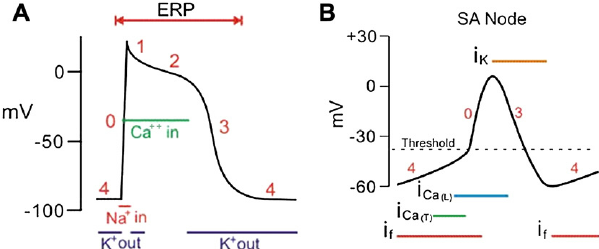
\includegraphics[width = 0.5\textwidth]{newactionpot}
\end{figure}

Ectopic firing---from a focus, not located at the Sinoatrial node, at which action potentials are initiated---can arise from 'afterdepolarisations': the free intracellular Ca$^{2+}$ concentration rises sharply during the depolarised phase of the action potential; when relaxation occurs, the concentration of Ca$^{2+}$  is reduced by uptake into the sarcoplasmic reticulum via Na$^{+}$/ Ca$^{2+}$  exchange. This is an electrogenic process: three Na$^{+}$ ions are exchanged for a single Ca$^{2+}$, thus making the potential difference more positive. This induces an inward current that can depolarise the cell which can lead to spontaneous action potentials firing \cite{Nattel2}. 



Atrial cell fibrosis causes cells to be unresponsive. Current research suggests that this is due to excessive Ca$^{2+}$ loading, which occurs with tachycardia as many action potentials are enacted. Furthermore, this leads to electrical remodelling of the heart, making AF the more probable pathway of activation regardless of the mechanism for tachycardia \cite{Nattel2}. Due to fibrillation, the concentration of the intracellular Ca$^{2+}$ is altered, thus impairing effective contraction which may give rise to blood clots that can cause strokes. %REVISEEE

%MONODOMAIN AND BIDOMAIN STUFF??

\section{\textbf{\underline{Types of Models}}} %METHODS

Mechanisms thought to be responsible for active cardiac arrhythmias are either enhanced/abnormal pulse formation or re-entry. For the former, simulations have included modelling the ionic currents of action potentials such as the Fenton-Karma model \cite{Grandi} \cite{Fenton} and modelling the impulse of an action potential using generic reaction-diffusion equations, such as the FitzHugh-Nagumo Model \cite{FitzHugh}. Most of these models are based on the pioneering work of Hodgkin and Huxley who described the action potential of the giant squid axon, which bears similarities to cardiac cells \cite{Hodgkin}. %CHECKKKKKKKKKKKKKKKKKKK
 For all of these models bidomain or monodomain approaches can be used to model the electrical propagation in myocardial tissue. % intracellularly????
  The bidomain model takes into account the anisotropy of intracellular and extracellular spaces. The monodomain model is a reduction of the bidomain model by assuming anisotropy ratios of intracellular and extracellular domains are equal---this is the model most commonly used in simulations today.%ET CETERA?
% ,   is the Many types of models have been used to simulate fibrillatory behaviour in the heart, from, and signals for contraction, to cellular automata and 

Re-entry---the mechanism by which a propagating impulse fails to die out after normal activation of the heart---has been studied in depth via various circus reentry formulations: the Ring Model, the Leading circle model, the Figure-of-Eight model and the Spiral Wave model \cite{Antze} \cite{Tusscher}. The Ring model models a wave of propagation that moves along one, unidirectional pathway of heart tissue and returns to the origin of excitation, thus simulating a central area of inexcitable tissue. This simple model implies that the conduction velocity and the refractory period are both factors: the length of the circuit (pathlength) must be greater or equal to the wavelength (the distance travelled by an impulse during the refractory period). The smaller the wavelength, the greater the number of reentry circuits that can be accommodated during the refractory period to promote fibrillatory behaviour. See figure 2(c).

The leading circle model found that there need not be a block of inexcitable tissue at the centre of circus movement for a reentry circuit to occur, using properly timed stimuli (see figure 2a). \cite{Allessie}. %Using a pathlength that is the size of the wavelength: decreased wavelength decreases minimum circuit size which increases number of circuits that can be accommodated.
 To rectify this reentry, it would be thought that the refractory period must increase to limit number of accommodated circuits, but incompatible observations have been found in antiarrhythmic drugs that block Na$^{+}$ channels, thus slowing down depolarisation. Such agents are effective in terminating AF, but according to leading circle theory should promote AF because they decrease conduction velocity and thereby decrease the wavelength. See figure 2(a) for diagram. 

The Figure of Eight model has a centre where two concurrently propagating waves circulate in opposite directions that merge into a common, central pathway. 

\begin{figure}
\caption[short title]{Diagram showing the leading circle and spiral wave models of reentry. PL = pathlength, RP = refractory period, CV = conduction velocity, WL = wavelength \cite{Nattel3}}
\centering
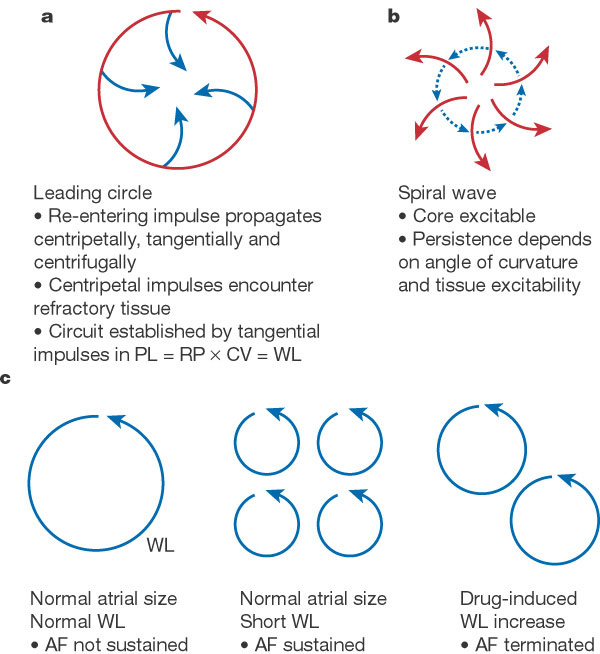
\includegraphics[width = 0.5\textwidth]{reeentry}
\end{figure}

The Spiral wave model---which consists of a single rotating wavefront around a core, simulating tachycardia---has been observed in systems that have sites that have excited, refractory and resting states in both homogeneous and heterogeneous media \cite{Greenburg} \cite{Bub}. This is due to anisotropies in conduction velocity in the cardiac tissue. See figure 2(b) and figure 3. % for comparison to a normal wavefront. 
 Experimental demonstration of spiral waves has been achieved by in research by Davidenko et al and the concept is now seen to be an underlying driver of fibrillation; the paradigm appears to more closely correspond with many clinical and experimental observations than other models \cite{Davidenko} \cite{Comtois}. In one such observation, the presence of rotors was seen in 96\% of patients with AF, in a 2012 study \cite{afstudy}. The curvature of the spiral wave is related to the speed of the wave, the more curvature the slower the speed of propagation. High curvature, and far-field instability, leads to spiral wave breakage into daughter wavelets. This agrees with
%popular classical modes of thought regarding the initiation of fibrillatory contraction, multiple circuit reentry, which in this case is due to spiral breakup, and 
recent opinions where single, small reentry circuits or local generators have been found to promote fibrillatory activity---the core of the spiral \cite{Skanes} \cite{Nattel2}. The tip of the spiral wave has been seen to drift around the core, thus moving the whole spiral wave. Such meandering can be a factor in promoting fibrillatory activity \cite{Tusscher}.
% Recent observations are in contradiction with the classical viewpoint,  . This is also concurrent 
 Extending the spiral wave model to 3D gives rise to scroll waves which propagate through multiple layers of cells and give rise to more complex wave dynamics and is therefore hard to implement computationally.  %It has been seen that the if a spiral wave is in homogenous media then it will always return to its resting state . 


\begin{figure}
\caption[short title]{Diagram showing a spiral wave reentry circuit. (a), a normal wavefront in the heart. (b) spiral wave, which simulates tachycardia, as can be seen by multiple propagating wavefronts in a small area. (c), turbulent activity due to break up of spiral wave giving rise to fibrillation \cite{Alonso}}
\centering
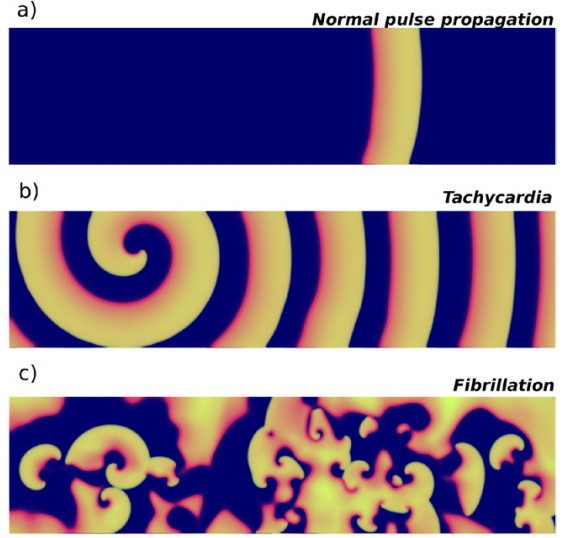
\includegraphics[width = 0.5\textwidth]{spiralbreak2tachy}
\end{figure}

\section{\textbf{\underline{Cellular Automata Models and}\\ \underline{Further Developments}}}



Cellular automaton models have been formulated as there is no need to simulate the exact shape of the action potential, based on differential equations, and it is high speed in large scale simulations \cite{Felipe}. Only relative properties such as the excitation wavefront, refractory period and the morphology of the heart need be considered. Cells' states depend only on the states of their neighbours: they are either at rest, become excited, or are refractory. Refractory cells revert to rest after the refractory period has elapsed.


Mainly square lattices have been used for such cellular automata models. One problem is isotropy, especially when spiral waves are simulated. As seen in research by Pourhasanzande et al, Moore, rather than Von Neumann, neighbourhoods can be used with a Markus model reducing the square shape of the spiral wave by choosing an appropriate threshold value of neighbours \cite{Pour}. See figure 4.


\begin{figure}
\caption[short title]{Diagram showing spiral wave generated by using (a)---a Moore neighborhood---and (b)---a Von
Neumann neighborhood showing the reduction of flat edges using the Moore model with the Markus method
 \cite{Pour}}
\centering
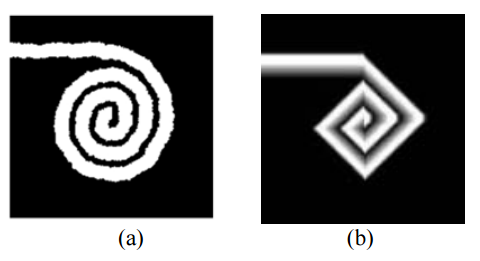
\includegraphics[width = 0.5\textwidth]{flatedgered}
\end{figure}

Recent research has shown that rotating wavefronts can be initiated in regions where the proportion of transverse coupling between strands of tissue is reduced to a critical value, leading to spontaneous fibrillatory activity, in contrast to normal 'linear' wavefronts. This can be seen in the rectilinear cellular automata model developed by Christensen et al and reflects current opinion: the fibrosis of cells, which reduces the coupling of electrical signals to other cells, leads to AF\cite{Christensen}. This research also supports targeted ablation to stop AF. Other studies suggest similar mechanisms such as the coupling of fibroblasts to atrial myocytes heterogeneously gives rise to spiral wave breakups \cite{Ozawa}.


In research by Fedotov, a cellular automaton model was constructed on the surface of a triangulated sphere to model spiral rotor waves on a closed, heterogeneous surface \cite{Fedotov}. It was shown that both a decrease in refractory period and conduction velocity from a "healthy" myocardium state, where no irregular excitation waves above 300bpm are observed, resulted in an area where spiral waves were formed. In addition, a multi-electrode system was created to study the localization of AF sources by simulated electrograms. 


More cellular automata models have been researched by Siregar et al, where a 3D model of the heart, with simplified morphology is simulated and, in addition, a 2D CA model is compared qualitative model \cite{Siregar} \cite{Siregar2}. A hybrid I/O cellular automata approach has also been studied in research by Bartocci et al to describe cardiac tissue and improve the efficiency of the simulation process by parallelization \cite{Bartocci}.

 The impact of left and right atrial tissue electrical heterogeneities to promote AF has been studied in a biophysical model and it was seen that AF is more persistent in the right atria \cite{Luca}. Further development could be achieved by simulation from a cellular automata perspective. Modelling scroll waves and replicating the morphology of the heart with its heterogeneities more closely seem to be viable directions for further research. The effects of antiarrhythmic drugs on the heart during AF can be studied, along with the associated mechanism by which proarrhythmia occurs, and methods for its rectification. Developing ways to find CFAEs with novel electrogram methods via simulation could help targeted ablation, stopping AF more effectively and efficiently. 



% Further developments could be obtained through this parallelization combined with 3D modelling, more accurately depicting the shape of the heart, making the code more efficient.

 %Many of these studies suggest targeted ablation can hinder or fully stop AF, therefore, electrogram-guided ablation to find CFAEs is a promising method it is concurrent with clinical observations. %electrogram-guided ablation to find CFAE.


%Most of these models only work one or two dimensionally, assuming that the heart is a 2D surface and not a 3D




%Cellular automaton models


%MAIN PAPER FROM KIM CHRISTIENSEN
%BIPOLAR ELECTROGRAM??
%METHODS TO POTENTIALLY STOP ATRIAL FIBRILLATION




%FUUUUUUUUUUUUURTHER METHODZZZZZZZZZZZZZZZZZZZZZZZZZZ




%\section{\textbf{\underline{Implications and Discussion}}}  %What our research project will be able to achieve, potentially



%\section{\textbf{\underline{Conclusion}}}




%In this literature review, possible underlying mechanisms of atrial fibrillation (AF) are described along with the relevant the electrophysiology of heart cells, specifically myocytes and  sinoatrial node cells. The integral role of these cells with regards to action potential propagation to contract the heart periodically is described. Models to simulate the action potentials of these cells to simulate reentry are seen to be a computationally costly way of modelling large scale cardiac tissue. Studied models of electrical wavefront propagation (reentry) that could cause AF, such as the ring, leading circle and spiral wave models are described; spiral wave reentry has been observed to be an underlying mechanism. Cellular automata---where cells' states change based on the states of their nearest neighbours---are viable models that reduce the amount of computation by not considering differential equations governing the action potentials. Therefore, reentry can be modelled on a large scale more easily. Moore neighbourhoods used with a Markus model can achieve smooth spiral waveforms that are isotropic and therefore model spiral wave reentry in a cellular automata models effectively. New directions of research can be taken to more accurately model AF such as: the morphology and heterogeneities of the heart, modelling 3D scroll wave dynamics and using hybrid I/O automata. 

\section{\textbf{\underline{Bibliography}}}
\begin{thebibliography}{7}

%####################################################
\bibitem{Hart}
Hart, R. G. \& Halperin, J. L. (2001).
\emph{Atrial fibrillation and stroke: concepts and controversies.},
Stroke 32, 803–808,
2001

\bibitem{Nattel1}
S. Nattel, 
\emph{ Experimental evidence for proarrhythmic mechanisms of antiarrhythmic drugs.}
Cardiovasc Res. 1998 Mar;37(3):567-77.

\bibitem{Tsui}
Tsui, S. S. L. Grace, A. A. Ludman, P. F. Schofield, P. M. Page, A. J. P. Rowland, E.  and Large, S. R., 
\emph{ Maze 3 for Atrial Fibrillation: Two Cuts Too Few?.}
 Pacing and Clinical Electrophysiology,
17: 2163–2166. doi:10.1111/j.1540-8159.1994.tb03819.x
1994


\bibitem{Greek}
Demosthenes G Katritsis, Ioannis Pantos and Efstathios P Efstathopoulos, 
\emph{Catheter ablation of atrial fibrillation guided by electrogram fractionation and dominant frequency analysis},
Expert Review of Cardiovascular Therapy 
Volume 9, 2011 - Issue 5, 631-636, 2014


\bibitem{Vincent}
V. DeCaprio, P. Hurzeler snd S. Furman, 
\emph{A Comparison of Unipolar and Bipolar Electrograms for Cardiac Pacemaker Sensing}
Circulation, Vol 56, No 5, November 1977
 

\bibitem{Augustus}
Augustus O. Grant, MB, ChB, PhD
\emph{Basic Science for the Clinical Electrophysiologist: Cardiac Ion Channels}
Circulation: Arrhythmia and Electrophysiology.
2009; 2: 185-194
doi: 10.1161/CIRCEP.108.789081

\bibitem{Nattel3}
Nattel S, Carlsson L.
\emph{ Innovative approaches to anti-arrhythmic drug therapy.},
Nat Rev Drug Discov. 2006; 5: 1034–1049. 


\bibitem{Mizzi}
\emph{Amiodarone supplants lidocaine in ACLS and CPR protocols}
A. Mizzi, T. Tran, D, Mangar, E. M. Camporesi
Anesthesiology Clinics 29(3):535-45 · September 2011


\bibitem{Nattel2}
S. Nattel, 
\emph{New Ideas about atrial fibrillation 50 years on},
 NATURE | VOL 415 | 10 JANUARY 2002 |

\bibitem{Grandi}
E. Grandi, S. V. Pandit, N. Voigt, M.D., A. J. Workman, D. Dobrev, J. Jalife, and D. M  Bers,
\emph{Human Atrial Action Potential and Ca$^{2+ }$ Model: Sinus Rhythm and Chronic Atrial Fibrillation},
Circ Res. 2011 October 14; 109(9): 1055–1066. doi:10.1161/CIRCRESAHA.111.253955.
November 2011

\bibitem{Fenton}
F. Fenton and A. Karma
\emph{Vortex dynamics in three-dimensional continuous myocardium with fiber
rotation: Filament instability and fibrillation},
1997

\bibitem{FitzHugh}
Richard FitzHugh, 
\emph{Impulses and Physiological States in Theoretical Models of Nerve Membrane},
Biophys J. 1961 Jul; 1(6): 445–466.


\bibitem{Hodgkin}
A. L. Hodgkin and A. F. Huxley, 
\emph{A quantitative description of membrane current and its application to conduction and excitation in nerve},
J. Physiol. (I952) I I7, 500-544

\bibitem{Antze}
 C. Antzelevitch
\emph{Basic mechanisms of re-entrant arrhythmias}
Curr Opin Cardiol. 2001 Jan;16(1):1-7.


\bibitem{Tusscher}
\emph{Spiral wave dynamics and ventricular arrhythmias},
 K. H. W. Johanna ten Tusscher,
 November 2004.

\bibitem{Allessie}
Allessie MA, Bonke FIM, Schopman JG,
\emph{ Circus movement in rabbit atrial muscle as a mechanism of tachycardia. III. The “leading circle” concept: a new model of circus movement in cardiac tissue without the involvement of an anatomical obstacle.},
 Circ Res 1977, 41:9–18.

\bibitem{Greenburg}
J. M. Greenberg and S. P. Hastings, 
\emph{Spatial Patterns for Discrete Models of Diffusion in Excitable Media}, 
SIAM J. APPL. MATH.
Vol. 34, No. 3, May 1978

\bibitem{Bub}
G. Bub, A. Shrier, and L. Glass,
\emph{Spiral Wave Generation in Heterogeneous Excitable Media},
 Phys. Rev. Lett.88, 058101 (2002)

\bibitem{Davidenko}
Davidenko JM, Kent PF, Chialvo DR, Michaels DC, Jalife J., 
\emph{Sustained vortex-like waves in normal isolated ventricular muscle.},
 Proc Natl Acad Sci USA. 1990;87:8785–8789

\bibitem{Comtois}
P. Comtois, J. Kneller, S. Nattel,
\emph{Of circles and spirals: Bridging the gap between the leading circle and spiral wave concepts of cardiac reentry}
Europace. 2005 Sep;7 Suppl 2:10-20.
DOI: http://dx.doi.org/10.1016/j.eupc.2005.05.011

\bibitem{afstudy}
S. M. Narayan, D. E. Krummen, and W.-J. RAPPEL, 
\emph{Clinical mapping approach to diagnose
electrical rotors and focal impulse sources for human atrial fibrillation},
 Journal of
cardiovascular electrophysiology, vol. 23, no. 5, pp. 447–454, 2012.



\bibitem{Skanes}
Mandapati, R., Skanes, A., Chen, J., Berenfeld, O. and  Jalife, J. 
\emph{Stable microreentrant sources as a mechanism of atrial fibrillation in the isolated sheep heart.}
Circulation 101, 194–199 (2000). 

\bibitem{Alonso}
S. Alonso, M. Bar and B. Echebarria
\emph{Nonlinear physics of electrical wave
propagation in the heart: a review},
Rep. Prog. Phys. 79 (2016) 096601, 
doi:10.1088/0034-4885/79/9/096601

\bibitem{Christensen}
Kim Christensen, Kishan A. Manani, and Nicholas S. Peters
\emph{Simple Model for Identifying Critical Regions in Atrial Fibrillation}
Phys. Rev. Lett. 114, 028104 – Published 16 January 2015

\bibitem{Ozawa}
Ashihara T, Haraguchi R, Nakazawa K, Namba T, Ikeda T, Nakazawa Y, Ozawa T, Ito M, Horie M, Trayanova NA., 
\emph{The role of fibroblasts in complex fractionated electrograms during persistent/permanent atrial fibrillation: implications for electrogram-based catheter ablation.}
Circ Res. 2012 Jan 20;110(2):275-84. doi: 10.1161/CIRCRESAHA.111.255026

\bibitem{Felipe}
F.A. Atienza, J. R. Carrion, A. G. Alberola, J. L. R. Alvarez, J. J. S. Munoz, J. M. Sanchez, M. V. Chavarri,
\emph{A Probabilistic Model of Cardiac Electrical Activity Based on a Cellular Automata System},
Revista Española de Cardiología (English Edition), Volume 58, Issue 1, January 2005, Pages 41-47,
doi:10.1016/S1885-5857(06)60233-8

\bibitem{Pour}
F. Pourhasanzande, S. H. Sabzpoushan
\emph{A new Cellular Automata Model of Cardiac
Action Potential Propagation based on
Summation of Excited Neighbors}, 
International Journal of Medical, Health, Biomedical, Bioengineering and Pharmaceutical Engineering Vol:4, No:8, 2010  

\bibitem{Fedotov}
N. M. Fedotov,  A. I. Oferkin, and S. V. Zhary,
\emph{Modeling Sources of Atrial Fibrillation on a Triangulated Sphere}
Biomedical Engineering, Vol. 49, No. 2, July, 2015, pp. 112115. 

\bibitem{Siregar}
P. Siregar, J. P. Sinteff, N. Julen, P. Le Beux,
\emph{An Interactive 3D Anisotropic Cellular Automata Model of the Heart}
Computers and Biomedical Research
Volume 31, Issue 5, October 1998, Pages 323-347, 
doi:10.1006/cbmr.1998.1485

\bibitem{Siregar2}
P. Siregar, J.P. Sinteff, M. Chahine, P. Lebeux
\emph{A Cellular Automata Model of the Heart and Its Coupling with a Qualitative Model}, 
Computers and Biomedical Research
Volume 29, Issue 3, June 1996, Pages 222-246,
doi:10.1006/cbmr.1996.0017

\bibitem{Bartocci}
E. Bartocci, F. Corradini, M.R. Di Berardini, E. Entcheva and S.A. Smolka, R. Grosu, 
\emph{Modeling and simulation of cardiac tissue using hybrid I/O automata}
Theoretical Computer Science
Volume 410, Issues 33–34, 21 August 2009, Pages 3149-3165,
doi:10.1016/j.tcs.2009.02.042


\bibitem{Luca}
A. Luca, V. Jaquemet, N. Virag, J. M. Vesin
\emph{Influence of Right and Left Atrial Tissue Heterogeneity on
Atrial Fibrillation Perpetuation }
Computing in Cardiology 2015; 42:449-452. 

%imref https://o.quizlet.com/i/1UZTM_D5PFefI8E5JOk8Ig_m.jpg


\end{thebibliography}


\end{document}